\documentclass[tikz,border=3pt]{standalone}
\usepackage[utf8]{inputenc}
\usepackage[T1]{fontenc}
\usepackage{lmodern}
\renewcommand{\familydefault}{\sfdefault}
\usepackage{sansmath}\sansmath
\usepackage{chemfig}
\usepackage{pgfplots}\pgfplotsset{compat=1.18,/pgf/number format/use comma,/pgf/number format/1000 sep={.}}
\usetikzlibrary{arrows.meta,calc,positioning,decorations.pathmorphing,patterns}
% paleta del sitio
\definecolor{nar}{HTML}{E8680C}\definecolor{narc}{HTML}{FFB35C}\definecolor{hielo}{HTML}{FFF3E8}
\definecolor{tinta}{HTML}{1D1D1F}\definecolor{gris}{HTML}{6E6E73}\definecolor{lila}{HTML}{7C5CF0}
\definecolor{azul}{HTML}{2F6FD6}\definecolor{menta}{HTML}{17A673}\definecolor{coral}{HTML}{E8342A}
\begin{document}
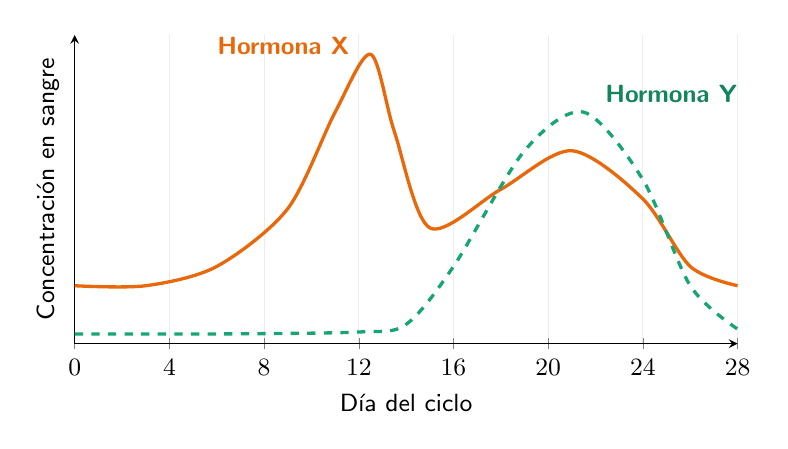
\begin{tikzpicture}[font=\small]
\begin{axis}[width=10cm,height=5.5cm,xmin=0,xmax=28,ymin=0,ymax=32,axis lines=left,ytick=\empty,xtick={0,4,...,28},
 xlabel={Día del ciclo},ylabel={Concentración en sangre},grid=major,grid style={gray!15},clip=false]
\addplot[nar,very thick,smooth] coordinates {(0,6)(3,6)(6,8)(9,14)(11,24)(12.5,30)(13.5,22)(15,12)(18,16)(21,20)(24,15)(26,8)(28,6)};
\addplot[menta,very thick,smooth,dashed] coordinates {(0,1)(6,1)(12,1.2)(14,2)(16,8)(19,20)(21.5,24)(24,17)(26,6)(28,1.5)};
\node[text=nar,font=\small\bfseries,anchor=south east] at (axis cs:12,29) {Hormona X};
\node[text=menta!80!black,font=\small\bfseries,anchor=south west] at (axis cs:22,24) {Hormona Y};
\end{axis}
\end{tikzpicture}
\end{document}
